\chapter{Metric Learning}\label{ch:metric-learning}
Molti algoritmi di machine learning si basano su una misura di distanza tra i dati: due esempi vicini nello spazio vengono considerati simili. In questo capitolo partiamo da due algoritmi di questo tipo, il KNN e il K-means, e dalle misure di distanza più usate. Poi vediamo il \textbf{metric learning}, ovvero come imparare dai dati una rappresentazione in cui una distanza fissata a priori funziona bene. Lo faremo prima con una trasformazione lineare e poi con una rete neurale (\emph{deep metric learning}).

\section{Algoritmi basati sulle distanze}
Diversi approcci di machine learning richiedono una misura di distanza tra punti in uno spazio $\mathbb{R}^d$, i cui punti rappresentano i dati del problema. Nel capitolo~\ref{ch:addestramento-cnn} abbiamo visto che una rete pre-addestrata, senza l'ultimo layer, è un feature extractor. Possiamo quindi calcolare le distanze non sui dati grezzi, ma sulle loro rappresentazioni $\phi(x)$, dove $\phi$ è una \textbf{representation function} (ad esempio appresa da una rete).

\subsection{K-Nearest Neighbor}
Il classificatore \textbf{nearest neighbor} si basa su un'idea semplice: dato un nuovo esempio $x'$, cerchiamo l'esempio del training set più vicino e gli assegniamo la stessa classe. L'ipotesi è che elementi vicini nello spazio della rappresentazione siano probabilmente simili. Pensiamo a MNIST: se l'immagine di una cifra è molto vicina a un'immagine del training set etichettata come 7, è probabile che sia anch'essa un 7.

Per misurare quanto due esempi sono simili ci serve una funzione di distanza $D(x, x')$, che deve essere piccola per esempi simili. La scelta più comune è la distanza euclidea:
\[
D(x, x') = \|x - x'\|_2 = \sqrt{\sum_{i=1}^{d} (x_i - x'_i)^2}.
\]
Il classificatore assegna a $x'$ la classe dell'esempio del training set più vicino:
\[
h(x') = y^{(j)}, \qquad j = \arg\min_{i} D\big(x', x^{(i)}\big)
\]
dove $x^{(j)}$ è il \textbf{nearest neighbor} di $x'$ e $y^{(j)}$ la sua etichetta. Questo algoritmo si chiama nearest neighbor, o \textbf{1-NN}. L'algoritmo~\ref{alg:1nn} lo riporta nella versione vista a lezione, in cui la distanza è calcolata sulle rappresentazioni $\phi$.

\begin{algorithm}[htbp]
\caption{Classificazione 1-NN}\label{alg:1nn}
\begin{algorithmic}[1]
\Require matrice $X$ ($m \times d$) dei campioni $\{x^{(i)}\}_{i=1}^m$, representation function $\phi$, vettore $y$ ($m \times 1$) delle etichette, con $y^{(i)} \in C$ (l'insieme delle classi), nuovo pattern $P$ da classificare
\Ensure classe del pattern $P$
\For{$i = 1, \dots, m$}
    \State $\mathrm{distanze}(i) \gets D\big(\phi(x^{(i)}), \phi(P)\big)$
\EndFor
\State $\mathrm{min\_index} \gets$ indice della distanza minima in $\mathrm{distanze}$
\State \Return $y^{(\mathrm{min\_index})}$
\end{algorithmic}
\end{algorithm}

\paragraph{Da 1-NN a K-NN.}
Il nearest neighbor funziona bene se gli esempi della stessa classe sono vicini tra loro nello spazio della rappresentazione. Spesso, però, il training set contiene degli \textbf{outlier}, ovvero esempi che non seguono la distribuzione degli altri. Può succedere perché i dati non sono puliti (un esempio etichettato male) oppure perché la rappresentazione non è ideale. Ad esempio, in MNIST potremmo avere un 1 scritto in modo da sembrare un 7. Se il nearest neighbor di un nuovo 7 è proprio quell'1, il 1-NN sbaglia, anche se tutti gli altri esempi vicini sono dei 7.

Conviene quindi guardare un intorno del punto, invece del solo punto più vicino. Fissare un raggio per l'intorno non è semplice: se lo spazio non è uniformemente denso, intorni con lo stesso raggio possono contenere numeri di elementi molto diversi, a volte anche nessuno. Si considerano quindi i $K$ esempi più vicini, dove $K$ è un iperparametro. Il classificatore \textbf{K-Nearest Neighbor} (K-NN) assegna la classe più frequente tra questi:
\[
h(x') = \mathrm{mode}\big\{y^{(i)} : x^{(i)} \in N_K(x')\big\}
\]
dove $N_K(x')$ è l'insieme dei $K$ esempi del training set più vicini a $x'$, e $\mathrm{mode}$ è la moda statistica, ovvero restituisce l'elemento più frequente di un insieme. Il 1-NN visto prima è il caso $K = 1$. In figura~\ref{fig:knn}, ad esempio, con $K = 3$ il pattern da classificare viene assegnato alla classe 1.

\begin{figure}[htbp]
\centering
\begin{widget}{knn}[k=3, query={3.0, 1.0}]
\begin{tikzpicture}[font=\scriptsize,
  c1/.style={draw=Accent, thick, circle, minimum size=2.5mm, inner sep=0pt},
  nuovo/.style={draw, fill=TextGray!30, minimum size=2.8mm, inner sep=0pt}]
  \foreach \x/\y in {2.6/1.7, 2.45/0.75, 3.0/0.35, 1.6/2.0} \node[c1] at (\x,\y) {};
  \foreach \x/\y in {0.4/1.6, 1.0/1.3, 0.5/0.6, 1.6/0.7, 1.4/-0.1, 2.0/0.2} {
    \draw[ObsColor, thick] (\x-0.08,\y-0.08) -- (\x+0.08,\y+0.08) (\x-0.08,\y+0.08) -- (\x+0.08,\y-0.08);
  }
  \node[nuovo] (p) at (3.0,1.0) {};
  \draw[dashed, TextGray] (p) circle (0.85);
  % legenda
  \node[nuovo] (l1) at (4.6,1.6) {};
  \node[right] at (l1.east) {pattern da classificare};
  \node[c1] (l2) at (4.6,1.1) {};
  \node[right] at (l2.east) {classe 1};
  \draw[ObsColor, thick] (4.52,0.52) -- (4.68,0.68) (4.52,0.68) -- (4.68,0.52);
  \node[right] at (4.7,0.6) {classe 2};
\end{tikzpicture}
\end{widget}
\caption{Classificazione K-NN con $K = 3$. I tre vicini del pattern da classificare (dentro il cerchio tratteggiato) appartengono tutti alla classe 1, che è quindi la classe assegnata.}
\label{fig:knn}
\end{figure}

Il valore di $K$ si può fissare in modo arbitrario oppure ottimizzare con un validation set o con la cross-validation. $K$ controlla come viene partizionato lo spazio: con $K$ piccolo il decision boundary segue ogni singolo punto (outlier compresi), mentre con $K$ grande le regioni diventano più regolari. È il solito trade-off tra bias e varianza.

Il KNN è un algoritmo supervisionato, perché usa le etichette del training set. Non ha però una vera fase di training: è un metodo \textbf{con memoria}, che salva tutto il training set e calcola le distanze solo quando deve classificare un nuovo esempio.

\paragraph{Curse of dimensionality.}
Il KNN funziona molto bene su dati con poche feature, ma soffre della \textbf{curse of dimensionality} (maledizione della dimensionalità). Al crescere del numero di dimensioni i dati diventano sparsi, e la distanza dal punto più vicino e quella dal punto più lontano diventano quasi uguali. Se tutti i punti sono ``ugualmente lontani'', il concetto di vicino perde di significato. Per questo, su dati ad alta dimensionalità come le immagini, conviene calcolare le distanze su una rappresentazione $\phi(x)$ compatta e non sui pixel.

\subsection{K-means}
Il \textbf{K-means} sfrutta la stessa idea per il \textbf{clustering}. In questo caso non abbiamo etichette (è un algoritmo non supervisionato), e vogliamo dividere automaticamente i dati in $K$ gruppi (o cluster) di elementi vicini tra loro. L'output è quindi una partizione dello spazio di input. L'algoritmo~\ref{alg:kmeans} riporta la versione vista a lezione.

\begin{algorithm}[htbp]
\caption{Clustering K-means}\label{alg:kmeans}
\begin{algorithmic}[1]
\Require matrice $X$ ($m \times d$) dei campioni, representation function $\phi$, numero di cluster $K$
\Ensure $K$ cluster (una partizione dello spazio di input)
\State scegli in modo casuale $K$ campioni di $X$ e usa le loro rappresentazioni come centroidi $\{c_1, \dots, c_K\}$
\Repeat
    \For{ogni campione $x^{(i)}$}
        \State trova il centroide $c_j$ più vicino, con la distanza $D$ tra $c_j$ e $\phi(x^{(i)})$
        \State assegna $x^{(i)}$ al cluster $j$
    \EndFor
    \For{ogni cluster $j$}
        \State ricalcola $c_j$ come media dei $\phi(x^{(i)})$ dei punti assegnati al cluster $j$
    \EndFor
\Until{convergenza, oppure per un numero fissato di iterazioni}
\end{algorithmic}
\end{algorithm}

Ogni iterazione ha due passi. Nel primo, ogni punto viene assegnato al cluster del centroide più vicino, secondo la distanza $D$. Nel secondo, ogni centroide viene ricalcolato come la media delle rappresentazioni dei punti che gli sono stati assegnati. Tornando a MNIST, con $K = 10$ vorremmo che ogni cluster raccogliesse le immagini di una sola cifra. Anche qui, quanto bene funziona dipende dalla distanza e dalla rappresentazione $\phi$ che usiamo.

\subsection{Misure di distanza}
In pratica si usano metriche standard quando si hanno conoscenze a priori sul dominio. Per gli spazi euclidei le più usate sono la distanza euclidea e la similarità del coseno:
\[
E(x^{(1)}, x^{(2)}) = \sqrt{\sum_i \big(x_i^{(1)} - x_i^{(2)}\big)^2}, \qquad
C(x^{(1)}, x^{(2)}) = \frac{\sum_i x_i^{(1)} x_i^{(2)}}{\sqrt{\sum_i \big(x_i^{(1)}\big)^2}\,\sqrt{\sum_i \big(x_i^{(2)}\big)^2}}.
\]
Per le distribuzioni di probabilità si usano invece la KL divergence (Kullback-Leibler)\footnote{La KL divergence non è simmetrica, ovvero in generale $D_{KL}(x^{(1)}, x^{(2)}) \neq D_{KL}(x^{(2)}, x^{(1)})$. A rigore, quindi, non è una distanza.} e il coefficiente di Bhattacharyya:
\[
D_{KL}(x^{(1)}, x^{(2)}) = \sum_i x_i^{(1)} \log \frac{x_i^{(1)}}{x_i^{(2)}}, \qquad
B(x^{(1)}, x^{(2)}) = \sum_i \sqrt{x_i^{(1)} x_i^{(2)}}.
\]
Attenzione all'interpretazione dei valori (tabella~\ref{tab:distanze}). La distanza euclidea e la KL divergence valgono 0 per esempi simili, e crescono per esempi dissimili. Il coseno e il coefficiente di Bhattacharyya, invece, sono misure di similarità: valgono 1 per esempi simili e diminuiscono per esempi dissimili.

\begin{table}[htbp]
\centering
\small
\begin{tabular}{@{}llccc@{}}
\toprule
Misura & Dominio & Intervallo & Simili & Dissimili \\
\midrule
Euclidea $E$ & spazi euclidei & $[0, +\infty)$ & 0 & $\to +\infty$ \\
Coseno $C$ & spazi euclidei & $[-1, 1]$ & 1 & $-1$ \\
KL divergence $D_{KL}$ & distribuzioni & $[0, +\infty)$ & 0 & $\to +\infty$ \\
Bhattacharyya $B$ & distribuzioni & $[0, 1]$ & 1 & 0 \\
\bottomrule
\end{tabular}
\caption{Le misure di distanza (e di similarità) più usate, con l'intervallo dei valori e i valori tipici per esempi simili e dissimili.}
\label{tab:distanze}
\end{table}

Tuttavia è spesso difficile stabilire quale sia la metrica più adatta per uno specifico problema o dataset. Qui entra in gioco il metric learning.

\section{Metric learning}
\begin{definizione}[Metric learning]
Il \textbf{metric learning} ha l'obiettivo di costruire algoritmi che creano automaticamente misure di distanza specifiche per un task (\emph{task-specific}), a partire da dati supervisionati o weakly supervised.
\end{definizione}
La misura di similarità appresa potrà poi essere usata per vari problemi, ad esempio per la classificazione con il KNN o per il clustering con il K-means. In realtà, la procedura di apprendimento agisce sullo spazio di input: lo trasforma in modo che possa essere ``usato'' con una metrica definita a priori. In altre parole, l'algoritmo riceve i dati e una metrica, e restituisce una rappresentazione dei dati in cui quella metrica produce i risultati attesi (figura~\ref{fig:ml-schema}).

\begin{figure}[htbp]
\centering
\begin{tikzpicture}[>=Stealth, font=\scriptsize,
  box/.style={draw, align=center, minimum height=1.1cm}]
  \node (dati) at (0,0.4) {dati};
  \node (met) at (0,-0.4) {metrica};
  \node[box, text width=3.0cm] (alg) at (3.0,0) {algoritmo di ML\\per il metric learning};
  \node[box, text width=4.2cm, fill=Accent!8] (rap) at (7.6,0) {rappresentazione dei dati in cui la metrica di input produce i risultati attesi};
  \draw[->] (dati) -- (alg.west |- dati);
  \draw[->] (met) -- (alg.west |- met);
  \draw[->] (alg) -- (rap);
\end{tikzpicture}
\caption{Lo schema del metric learning. L'algoritmo riceve i dati e una metrica definita a priori, e trasforma i dati in modo che la metrica funzioni.}
\label{fig:ml-schema}
\end{figure}

\subsection{Supervised e weakly supervised}
Ci sono due categorie principali di metric learning:
\begin{itemize}
    \item \textbf{Supervised}: l'algoritmo ha accesso a dati etichettati, in cui a ogni dato è associata un'etichetta di classe. L'obiettivo è trasformare lo spazio dei dati di input in modo che i punti con la stessa etichetta risultino vicini nel nuovo spazio, e i punti con etichette diverse risultino lontani.
    \item \textbf{Weakly supervised}: l'algoritmo ha accesso a dati in cui la supervisione è solo a livello di tuple (coppie, triplette, eccetera), ad esempio coppie simili e coppie dissimili. L'obiettivo è trasformare lo spazio in modo che le tuple simili siano vicine nello spazio di output, e quelle dissimili lontane.
\end{itemize}
Un esempio di weakly supervised sono le facce sorridenti. Non abbiamo un'etichetta di classe per ogni faccia, ma sappiamo che due facce sorridenti formano una coppia simile, mentre una faccia sorridente e una non sorridente formano una coppia dissimile.

Il problema del metric learning si formula quindi come un problema di ottimizzazione: bisogna trovare i parametri di una trasformazione dello spazio di input, rispetto a una misura di distanza. Si minimizza una funzione obiettivo sui dati di input.

\subsection{Mahalanobis distance learning}
Il caso più semplice è una trasformazione lineare. Nel \textbf{Mahalanobis distance learning} (implementato ad esempio in scikit-learn) la distanza tra due esempi è:
\[
D(x^{(1)}, x^{(2)}) = \sqrt{\big(Lx^{(1)} - Lx^{(2)}\big)^T \big(Lx^{(1)} - Lx^{(2)}\big)}
\]
dove $x \in \mathbb{R}^d$ è il vettore delle feature e $L \in \mathbb{R}^{m \times d}$ è la matrice dei parametri. Si cerca una trasformazione lineare $L$ dello spazio delle feature che soddisfi l'obiettivo del metric learning (supervised o weakly supervised). Ad esempio, vogliamo che i pattern simili abbiano distanza 0 e quelli dissimili distanza 1. Il nome viene dal fatto che, ponendo $M = L^T L$, la distanza si può riscrivere come $\sqrt{(x^{(1)} - x^{(2)})^T M\, (x^{(1)} - x^{(2)})}$, che è proprio la forma della distanza di Mahalanobis.

$L$ trasforma un vettore di $d$ componenti in uno di $m$ componenti (figura~\ref{fig:mahalanobis}). Se $m < d$, quindi, otteniamo anche una riduzione di dimensionalità. Se invece $L$ è la matrice identità, $D$ non è altro che la distanza euclidea.

\begin{figure}[htbp]
\centering
\begin{tikzpicture}[>=Stealth, font=\scriptsize]
  \draw[fill=Accent!12] (0,-0.6) rectangle (2.0,0.6);
  \node at (1.0,0) {$L$};
  \node[left] at (0,0) {$m$};
  \node[above] at (1.0,0.6) {$d$};
  \draw[fill=TextGray!15] (2.4,-1.0) rectangle (2.75,1.0);
  \node at (2.575,0) {$x$};
  \node[right] at (2.75,0.7) {$d$};
  \node[below] at (2.575,-1.0) {1};
  \draw[->, thick] (3.3,0) -- (4.1,0);
  \draw[fill=Accent!25] (4.4,-0.6) rectangle (4.75,0.6);
  \node[right] at (4.75,0) {$m$};
  \node[below] at (4.575,-0.6) {1};
\end{tikzpicture}
\caption{La trasformazione lineare del Mahalanobis distance learning: la matrice $L$ ($m \times d$) trasforma il vettore delle feature $x$ ($d \times 1$) in un vettore $Lx$ ($m \times 1$). Con $m < d$ si ha una riduzione di dimensionalità.}
\label{fig:mahalanobis}
\end{figure}

Restano due domande. Come possiamo trasformare lo spazio di input, ovvero come troviamo $L$? E se volessimo trasformazioni non lineari? La risposta è la stessa: con un'architettura neurale.

\section{Deep metric learning}
\subsection{L'idea di partenza}
Nel \textbf{deep metric learning} la trasformazione è una rete neurale $L_\vartheta$ (figura~\ref{fig:dml-idea}). Due esempi $x^{(1)}$ e $x^{(2)}$ passano attraverso la stessa rete, che li trasforma in $\tilde{x}^{(1)}$ e $\tilde{x}^{(2)}$:
\[
\tilde{x} \equiv L_\vartheta(x).
\]
Sulle rappresentazioni trasformate calcoliamo la distanza $D$, e con questa una funzione di loss. Le coppie $(x^{(1)}, x^{(2)})$ sono etichettate come simili (1) oppure dissimili (0). Nel caso supervised, ad esempio, sono simili due campioni della stessa classe e dissimili due campioni di classi diverse. La distanza $D$ stabilisce l'errore utile per aggiornare i parametri dell'architettura $L_\vartheta$.

\begin{figure}[htbp]
\centering
\begin{tikzpicture}[>=Stealth, font=\small]
  \node (x1) at (0,0.45) {$x^{(1)}$};
  \node (x2) at (0,-0.45) {$x^{(2)}$};
  \draw[fill=Accent!12] (1.0,-0.9) -- (1.0,0.9) -- (2.2,0.5) -- (2.2,-0.5) -- cycle;
  \node at (1.6,0) {$L_\vartheta$};
  \node (t1) at (3.2,0.45) {$\tilde{x}^{(1)}$};
  \node (t2) at (3.2,-0.45) {$\tilde{x}^{(2)}$};
  \node[draw, circle, inner sep=2pt] (d) at (4.4,0) {$D$};
  \node[right] (l) at (5.3,0) {$\mathrm{loss}\big(\tilde{x}^{(1)}, \tilde{x}^{(2)}, D\big)$};
  \draw[->] (x1) -- (1.0,0.45);
  \draw[->] (x2) -- (1.0,-0.45);
  \draw[->] (2.2,0.45) -- (t1);
  \draw[->] (2.2,-0.45) -- (t2);
  \draw[->] (t1) -- (d);
  \draw[->] (t2) -- (d);
  \draw[->] (d) -- (l);
\end{tikzpicture}
\caption{L'idea alla base del deep metric learning. La rete $L_\vartheta$ trasforma i due esempi, e la loss confronta le rappresentazioni trasformate tramite la distanza $D$.}
\label{fig:dml-idea}
\end{figure}

Ci servirà capire tre cose:
\begin{enumerate}
    \item chi è $L_\vartheta$: una rete neurale.
    \item chi è $D$, ovvero come scrivere una funzione di loss che tenga conto di $D$, al fine di ottenere una buona $L_\vartheta$.
    \item come campionare le tuple per ottimizzare i parametri, sia nel caso supervised che in quello weakly supervised.
\end{enumerate}
Il nuovo spazio $\tilde{X}$, ottenuto dopo la trasformazione, viene generalmente chiamato \textbf{embedding space}. In fase di test usiamo $L_\vartheta$ per trasformare il nuovo pattern, e $D$ per cercare il pattern più vicino nello spazio trasformato del training set.

\subsection{Approcci contrastive}
Gli approcci \textbf{contrastive} cercano una loss function che spinga direttamente gli elementi simili a essere vicini nello spazio, e quelli dissimili a essere lontani. La misura di distanza generalmente usata per costruire l'embedding space negli approcci contrastive è la distanza euclidea $\ell_2$:
\[
D(p^{(1)}, p^{(2)}) = \|p^{(1)} - p^{(2)}\|_2 = \sqrt{\sum_i \big(p_i^{(1)} - p_i^{(2)}\big)^2}.
\]
L'obiettivo è ottimizzare, con una loss function opportuna, un'architettura $L_\vartheta$ tale che la distanza dopo la trasformazione
\[
D\big(L_\vartheta(p^{(1)}), L_\vartheta(p^{(2)})\big)
\]
rispetti i requisiti: simili vicini e dissimili lontani.

In genere $L_\vartheta$ è un'architettura nota, che ottiene buoni risultati in problemi di classificazione (ad esempio VGG o ResNet) o di regressione (ad esempio PoseNet). Si può anche partire da un modello pre-addestrato, come abbiamo visto con il transfer learning.

\subsection{Contrastive loss}
La \textbf{contrastive loss} è una loss function classica, proposta da Chopra et al. nel 2005 \cite{Chopra2005}. Siano $x^{(1)}$ e $x^{(2)}$ due campioni del dataset, con etichette $y^{(1)}$ e $y^{(2)}$. Sia inoltre $\mathbf{1}_A$ la funzione indicatrice, che restituisce 1 se il predicato $A$ è vero e 0 se è falso.

\begin{definizione}[Contrastive loss]
La contrastive loss, da minimizzare, è definita come:
\begin{align*}
\mathrm{loss}_{\mathrm{contrastive}}(x^{(1)}, x^{(2)}, D) = \frac{1}{2}\Big[\, &\mathbf{1}_{y^{(1)} = y^{(2)}}\, D\big(L_\vartheta(x^{(1)}), L_\vartheta(x^{(2)})\big)^2 \\
+\, &\mathbf{1}_{y^{(1)} \neq y^{(2)}} \max\big(0,\ \alpha - D\big(L_\vartheta(x^{(1)}), L_\vartheta(x^{(2)})\big)\big)^2 \Big]
\end{align*}
dove $\alpha > 0$ è detto \textbf{margine}.
\end{definizione}

Per brevità scriviamo $D$ al posto di $D\big(L_\vartheta(x^{(1)}), L_\vartheta(x^{(2)})\big)$. Dei due termini ne resta sempre solo uno:
\begin{itemize}
    \item \textbf{Caso 1}, campioni simili: si considera $\frac{1}{2}D^2$. Quindi minimizziamo la distanza euclidea tra i simili.
    \item \textbf{Caso 2}, campioni dissimili: si considera $\frac{1}{2}\max(0, \alpha - D)^2$.
\end{itemize}

Vediamolo graficamente (figura~\ref{fig:contrastive}, a sinistra). Supponiamo che il cerchio e le stelle siano simili, mentre il cerchio e i quadrati siano dissimili. Vogliamo massimizzare le distanze \textbf{inter-class} (frecce tratteggiate) e minimizzare le distanze \textbf{intra-class} (frecce continue). Per ogni punto, quindi, vogliamo che la massima distanza intra-class sia più piccola della minima distanza inter-class.

Il margine $\alpha$ traduce questa richiesta (figura~\ref{fig:contrastive}, a destra). Dopo la trasformazione dello spazio, rispetto al punto preso in considerazione (il cerchio), tutte le stelle devono avere una distanza minore di $\alpha$, mentre tutti i quadrati devono avere una distanza maggiore. Se riusciamo a ottenere questo, la ricerca del vicino diventa semplice: se un nuovo punto da classificare sta a una distanza minore di $\alpha$ da un altro, allora i due sono simili, altrimenti sono dissimili.

\begin{figure}[htbp]
\centering
\begin{tikzpicture}[>=Stealth, font=\scriptsize,
  ancora/.style={draw, circle, thick, minimum size=3mm, inner sep=0pt},
  simile/.style={draw=LemmaColor, fill=LemmaColor!30, star, star points=5, star point ratio=2.25, minimum size=3.5mm, inner sep=0pt},
  dissimile/.style={draw=red!70!black, fill=red!15, minimum size=2.8mm, inner sep=0pt}]
  % a sinistra: le stelle vengono avvicinate, i quadrati allontanati
  \node[ancora] (o) at (0,0) {};
  \foreach \a in {150, 30, 265, 340} {
    \node[simile] (s) at (\a:1.7) {};
    \draw[->, thick, LemmaColor] (s) -- (\a:0.3);
  }
  \foreach \a in {90, 180, 225, 300} {
    \node[dissimile] (q) at (\a:1.7) {};
    \draw[->, dashed, red!70!black] (\a:0.3) -- (q);
  }
  % a destra: il margine alpha
  \begin{scope}[shift={(5.2,0)}]
    \draw[TextGray, fill=TextGray!6] (0,0) circle (1.2);
    \node[ancora] (o2) at (0,0) {};
    \node[simile] at (40:0.75) {};
    \node[simile] at (200:0.6) {};
    \node[dissimile] at (330:1.7) {};
    \node[dissimile] at (110:1.65) {};
    \draw[->, TextGray] (0,0) -- (250:1.2) node[midway, left] {$\alpha$};
  \end{scope}
  % legenda
  \node[simile] (l1) at (-1.4,-2.4) {};
  \node[right] at (l1.east) {simile al cerchio};
  \node[dissimile] (l2) at (1.4,-2.4) {};
  \node[right] at (l2.east) {dissimile dal cerchio};
\end{tikzpicture}
\caption{A sinistra, la contrastive loss avvicina i campioni simili (frecce continue) e allontana quelli dissimili (frecce tratteggiate). A destra, dopo il training: i simili stanno entro il margine $\alpha$ dal cerchio, i dissimili fuori.}
\label{fig:contrastive}
\end{figure}

Questo concetto è espresso proprio dal termine per i dissimili:
\[
\frac{1}{2}\max\big(0,\ \alpha - D\big)^2.
\]
La formula penalizza i punti dissimili la cui distanza $D$ è minore di $\alpha$: in questo caso $\alpha - D$ è positivo, e abbiamo un ``errore'' $(\alpha - D)^2$ da usare per aggiornare i pesi. Se invece la distanza è maggiore o uguale ad $\alpha$, $\alpha - D$ è negativo o nullo, e il massimo restituisce 0. Il gradiente è quindi nullo e i pesi non vengono aggiornati: i punti dissimili sono già a una distanza adeguata, e non li spingiamo ancora più lontano (figura~\ref{fig:margine-casi}).

\begin{figure}[htbp]
\centering
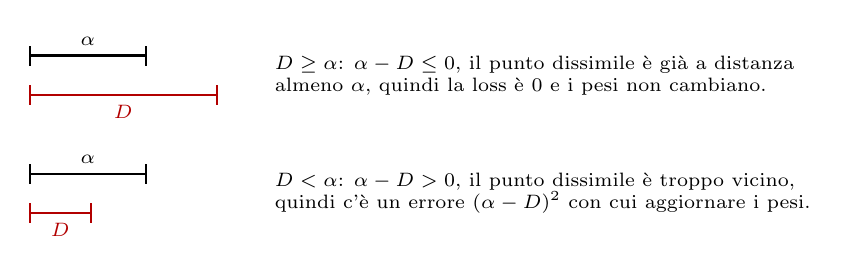
\begin{tikzpicture}[font=\scriptsize]
  \draw[|-|, thick] (0,0.3) -- (1.5,0.3) node[midway, above] {$\alpha$};
  \draw[|-|, thick, red!70!black] (0,-0.2) -- (2.4,-0.2) node[midway, below] {$D$};
  \node[right, align=left] at (3.0,0.05) {$D \ge \alpha$: $\alpha - D \le 0$, il punto dissimile è già a distanza\\almeno $\alpha$, quindi la loss è 0 e i pesi non cambiano.};
  \draw[|-|, thick] (0,-1.2) -- (1.5,-1.2) node[midway, above] {$\alpha$};
  \draw[|-|, thick, red!70!black] (0,-1.7) -- (0.8,-1.7) node[midway, below] {$D$};
  \node[right, align=left] at (3.0,-1.45) {$D < \alpha$: $\alpha - D > 0$, il punto dissimile è troppo vicino,\\quindi c'è un errore $(\alpha - D)^2$ con cui aggiornare i pesi.};
\end{tikzpicture}
\caption{I due casi del termine $\frac{1}{2}\max(0, \alpha - D)^2$ per una coppia di punti dissimili.}
\label{fig:margine-casi}
\end{figure}

Uno dei motivi per cui usiamo il margine è evitare che l'ottimizzazione prenda delle ``scorciatoie''. Senza un vincolo sui dissimili, la rete potrebbe mappare tutti i punti su un unico punto, con distanza zero tra ogni coppia dopo il training. Il termine con il margine lo impedisce, perché obbliga le coppie dissimili a restare almeno a distanza $\alpha$.

\subsection{Il caso weakly supervised}
Nella definizione della loss abbiamo supposto il caso supervised, in cui ogni pattern $x$ è associato a un'etichetta $y$. Nel caso weakly supervised non abbiamo etichette di classe, ma possiamo associare delle etichette alle coppie di punti (simili o dissimili).

Supponiamo, ad esempio, di voler costruire un algoritmo che, data un'immagine in input, cerchi in un dataset l'immagine più simile. Le immagini del dataset sono associate a delle coordinate, ovvero alla posizione e all'orientamento rispetto alla mappa di un ambiente (figura~\ref{fig:ambiente}, a sinistra). A una nuova immagine, acquisita nello stesso ambiente, vorremmo associare una posizione $(x, y)$ e un orientamento (supponiamo che tutte le immagini siano acquisite alla stessa altezza $z$). Un caso concreto è la localizzazione di un carrello della spesa all'interno di un supermercato.

Per farlo possiamo usare un KNN con $K = 1$: dopo aver addestrato la rete con una contrastive loss, cerchiamo l'immagine più simile usando la sua rappresentazione e la distanza euclidea $\ell_2$.

\begin{osservazione}
Le immagini di training hanno delle etichette relative alla posizione e all'orientamento, ma non sono etichette di classe. Non possiamo quindi valutare le condizioni della loss ($\mathbf{1}_{y^{(1)} = y^{(2)}}$ oppure $\mathbf{1}_{y^{(1)} \neq y^{(2)}}$): poiché campioniamo le immagini nell'ambiente, verosimilmente avremo $y^{(1)} \neq y^{(2)}$ per quasi tutte le coppie.
\end{osservazione}

Possiamo comunque sfruttare l'algoritmo con un \textbf{relabeling}: associamo a ogni coppia di immagini una similarità o una dissimilarità, cambiando la funzione indicatrice. Ad esempio:
\[
\mathbf{1}(y^{(1)}, y^{(2)}) =
\begin{cases}
1 & \text{se } \|p^{(1)} - p^{(2)}\| < t \text{ e } |o^{(1)} - o^{(2)}| < g \\
0 & \text{altrimenti}
\end{cases}
\]
dove $p$ è la posizione dell'immagine, $o$ il suo orientamento, mentre $t$ e $g$ sono parametri scelti dall'utente. Consideriamo quindi simile una coppia di immagini vicine nello spazio e con un orientamento simile (figura~\ref{fig:ambiente}, a destra).

\begin{figure}[htbp]
\centering
\begin{tikzpicture}[>=Stealth, font=\scriptsize]
  % ambiente: le pose delle immagini di training
  \draw (0,0) rectangle (4.4,2.6);
  \node[above] at (2.2,2.6) {ambiente};
  \foreach \x/\y/\a in {0.4/2.2/-60, 0.9/1.9/20, 1.6/2.1/-90, 2.4/2.2/-100, 3.1/2.0/-130, 3.8/2.2/200,
                        0.5/1.2/-30, 1.0/0.8/75, 1.5/1.3/30, 2.1/1.0/-80, 2.7/1.4/-70, 3.3/1.1/0,
                        3.9/1.3/-110, 0.7/0.4/45, 1.6/0.5/210, 2.9/0.5/100, 3.7/0.4/150} {
    \fill[TextGray] (\x,\y) circle (0.03);
    \draw[->, TextGray] (\x,\y) -- ++(\a:0.3);
  }
  \fill[Accent] (2.3,0.4) circle (0.04);
  \draw[->, thick, Accent] (2.3,0.4) -- ++(60:0.35);
  \draw[Accent] (2.4,0.5) circle (0.22);
  \draw[Accent] (2.4,0.28) -- (2.4,-0.4) node[below, draw, fill=white] {IMG};
  \node[right, align=left] at (4.5,1.3) {$p$, $o$: posizione e orientamento\\di un'immagine IMG\\acquisita in quel punto};
  % relabeling
  \begin{scope}[shift={(8.2,0.3)}]
    \draw (0,0) rectangle (2.6,2.0);
    \fill[LemmaColor] (0.4,0.5) circle (0.04);
    \draw[->, thick, LemmaColor] (0.4,0.5) -- ++(45:0.6);
    \fill[LemmaColor] (0.9,0.35) circle (0.04);
    \draw[->, thick, LemmaColor] (0.9,0.35) -- ++(35:0.6);
    \fill[red!70!black] (2.0,1.6) circle (0.04);
    \draw[->, thick, red!70!black] (2.0,1.6) -- ++(-70:0.6);
    \node[LemmaColor, below] at (0.7,0) {simili};
    \node[red!70!black, below] at (2.1,0) {dissimile};
  \end{scope}
\end{tikzpicture}
\caption{A sinistra, le immagini di training sono acquisite in diversi punti dell'ambiente, ognuna con una posizione e un orientamento (le frecce). A destra, il relabeling: due immagini vicine e con orientamento simile formano una coppia simile, mentre un'immagine lontana o con orientamento diverso è dissimile.}
\label{fig:ambiente}
\end{figure}

Nella loss usiamo la nuova definizione $\mathbf{1}(y^{(1)}, y^{(2)})$ per la parte che riguarda le coppie simili, e $1 - \mathbf{1}(y^{(1)}, y^{(2)})$ per la parte che riguarda le coppie dissimili. La loss function diventa quindi:
\begin{align*}
\mathrm{loss}_{\mathrm{contrastive}}(x^{(1)}, x^{(2)}, D) = \frac{1}{2}\Big[\, &\mathbf{1}(y^{(1)}, y^{(2)})\, D\big(L_\vartheta(x^{(1)}), L_\vartheta(x^{(2)})\big)^2 \\
+\, &\big(1 - \mathbf{1}(y^{(1)}, y^{(2)})\big) \max\big(0,\ \alpha - D\big(L_\vartheta(x^{(1)}), L_\vartheta(x^{(2)})\big)\big)^2 \Big].
\end{align*}

\subsection{Siamese network}
Un altro esempio weakly supervised sono le facce sorridenti, in cui la similarità si basa sul contenuto delle immagini. L'architettura usata in questi casi è la \textbf{siamese network} (figura~\ref{fig:siamese}). In realtà le architetture sono due, una per ogni elemento della coppia, ma condividono i pesi (\emph{shared weights}): sono quindi la stessa rete $L_\vartheta$ applicata due volte. Il backward pass attraversa i due rami separatamente, ma poiché i pesi sono condivisi, i due contributi del gradiente aggiornano gli stessi parametri.

\begin{figure}[htbp]
\centering
\begin{tikzpicture}[>=Stealth, font=\small]
  \foreach \y/\k in {0.9/1, -0.9/2} {
    \node (x\k) at (0,\y) {$x^{(\k)}$};
    \draw[fill=Accent!12] (0.8,\y-0.45) -- (0.8,\y+0.45) -- (1.8,\y+0.25) -- (1.8,\y-0.25) -- cycle;
    \node at (1.3,\y) {$L_\vartheta$};
    \node (l\k) at (3.2,\y) {$L_\vartheta(x^{(\k)})$};
    \draw[->] (x\k) -- (0.8,\y);
    \draw[->] (1.8,\y) -- (l\k);
  }
  \draw[<->, dashed, TextGray] (1.3,0.4) -- (1.3,-0.4) node[midway, right, font=\scriptsize] {pesi condivisi};
  \node[draw, circle, inner sep=2pt] (d) at (4.8,0) {$D$};
  \draw[->] (l1) -- (d);
  \draw[->] (l2) -- (d);
  \node[right] (loss) at (5.7,0) {$\mathrm{loss}_{\mathrm{contrastive}}$};
  \draw[->] (d) -- (loss);
  \node (y1) at (6.5,1.3) {$y^{(1)}$};
  \node (y2) at (6.5,-1.3) {$y^{(2)}$};
  \draw[->] (y1) -- (loss);
  \draw[->] (y2) -- (loss);
\end{tikzpicture}
\caption{Una siamese network. I due elementi della coppia passano attraverso due copie della stessa rete $L_\vartheta$, con pesi condivisi. La loss usa la distanza $D$ tra le due rappresentazioni e le etichette $y^{(1)}$ e $y^{(2)}$ (o la loro similarità).}
\label{fig:siamese}
\end{figure}

Il training procede così:
\begin{enumerate}[start=0]
    \item si fa il relabeling delle coppie di facce (simili o dissimili).
    \item si campionano delle coppie. Bisogna fare in modo che il campionamento consideri sia casi simili che casi dissimili, e anche casi ``difficili''.
    \item ogni pattern della coppia viene rappresentato tramite $L_\vartheta$, dove $L_\vartheta$ è un'architettura neurale (ad esempio VGG o ResNet).
    \item si valuta la funzione di loss usando la distanza $D$.
    \item si aggiornano i pesi di $L_\vartheta$ con la backpropagation.
\end{enumerate}

\subsection{Triplet loss}
Nella contrastive loss ogni coppia è simile oppure dissimile. Perché non guardare contemporaneamente un caso simile e uno dissimile? È l'idea della \textbf{triplet loss} (Schroff et al., 2015 \cite{Schroff2015}), una delle loss di metric learning più usate.

Siano $x^{(1)}$, $x^{(2)}$ e $x^{(3)}$ tre campioni del dataset tali che $y^{(1)} = y^{(2)}$ e $y^{(1)} \neq y^{(3)}$. In letteratura $x^{(1)}$ è detto \textbf{ancora} (\emph{anchor}), mentre $x^{(2)}$ è chiamato \textbf{campione positivo}, perché ha la stessa etichetta dell'ancora (è simile). $x^{(3)}$, infine, è detto \textbf{campione negativo}, perché ha un'etichetta diversa dall'ancora (è dissimile). Si considerano quindi triplette (ancora, positivo, negativo) per addestrare la rete $L_\vartheta$ che trasforma lo spazio delle feature.

\begin{definizione}[Triplet loss]
La triplet loss è definita come:
\[
\mathrm{loss}_{\mathrm{triplet}}(x^{(1)}, x^{(2)}, x^{(3)}, D) = \max\big(0,\ D_P - D_N + \alpha\big)
\]
dove $\alpha$ è il margine, mentre
\[
D_P = D\big(L_\vartheta(x^{(1)}), L_\vartheta(x^{(2)})\big)^2, \qquad D_N = D\big(L_\vartheta(x^{(1)}), L_\vartheta(x^{(3)})\big)^2
\]
sono le distanze (al quadrato) dell'ancora dal positivo e dal negativo.
\end{definizione}

Anche qui ci sono due casi:
\begin{itemize}
    \item \textbf{Caso 1}: $D_P - D_N + \alpha \le 0$, ovvero $D_P + \alpha \le D_N$. La distanza tra i dissimili è già maggiore della distanza tra i simili più il margine. Il massimo vale 0, e non è necessario aggiornare i pesi.
    \item \textbf{Caso 2}: $D_P - D_N + \alpha > 0$, ovvero $D_P + \alpha > D_N$. Il negativo è troppo vicino all'ancora, e vogliamo che venga allontanato con un errore pari a $D_P - D_N + \alpha$ (figura~\ref{fig:triplet}).
\end{itemize}

\begin{figure}[htbp]
\centering
\begin{widget}{triplet}[alpha=0.5]
\begin{tikzpicture}[>=Stealth, font=\scriptsize,
  ancora/.style={draw, circle, thick, minimum size=3mm, inner sep=0pt},
  simile/.style={draw=LemmaColor, fill=LemmaColor!30, star, star points=5, star point ratio=2.25, minimum size=3.5mm, inner sep=0pt},
  dissimile/.style={draw=red!70!black, fill=red!15, minimum size=2.8mm, inner sep=0pt}]
  \node[ancora, label=left:A] (a) at (0,0) {};
  \node[dissimile, label=above:N] (n) at (0.6,0.8) {};
  \node[simile, label=right:P] (p) at (1.4,-1.2) {};
  \draw[dashed, red!70!black] (a) -- (n) node[midway, left] {$D_N$};
  \draw[dotted, thick, LemmaColor] (a) -- (p) node[midway, left] {$D_P$};
  \draw[double, ->, thick] (2.5,0) -- (3.9,0) node[midway, above] {vorremmo};
  \begin{scope}[shift={(4.8,0)}]
    \node[ancora, label=left:A] (a2) at (0,0) {};
    \node[simile, label=right:P] (p2) at (0.5,-0.6) {};
    \node[dissimile, label=above:N] (n2) at (2.6,1.4) {};
    \draw[dashed, red!70!black] (a2) -- (n2) node[midway, above left] {$D_N$};
    \draw[dotted, thick, LemmaColor] (a2) -- (p2);
  \end{scope}
\end{tikzpicture}
\end{widget}
\caption{Il caso 2 della triplet loss. A sinistra il negativo N è più vicino all'ancora A del positivo P. Vorremmo invece che il positivo fosse vicino all'ancora e il negativo lontano, almeno di un margine $\alpha$ in più.}
\label{fig:triplet}
\end{figure}

Nei modelli basati sulla triplet loss conta molto il \textbf{campionamento dei negativi}. A ogni training step vogliamo campionare triplette $(x^{(1)}, x^{(2)}, x^{(3)})$ tali che $D_N < D_P + \alpha$, ovvero triplette che la nostra rete $L_\vartheta$ non mappa ancora nel modo voluto. Le altre hanno loss nulla, e non contribuiscono all'apprendimento.

La differenza principale tra la contrastive loss classica e la triplet loss sta nel fatto che, con quest'ultima, si ottimizza considerando contemporaneamente campioni positivi e negativi.

\subsection{Quadruplet loss}
Negli anni sono state proposte diverse altre varianti degli approcci contrastive. Tra queste c'è la \textbf{quadruplet loss} (Chen et al., 2017 \cite{Chen2017}), che cerca di massimizzare la variazione inter-class delle feature e di minimizzare quella intra-class. La triplet loss vista prima, infatti, non tiene conto della variazione delle feature all'interno della classe.

Data una quadrupla di campioni $x^{(1)}$, $x^{(2)}$, $x^{(3)}$, $x^{(4)}$ tali che $y^{(1)} = y^{(2)} = y^{(4)}$ e $y^{(1)} \neq y^{(3)}$, la loss è definita come segue\footnote{È la formulazione vista a lezione. Nel paper originale \cite{Chen2017} la quadrupla è formata da un'ancora $x_i$, un positivo $x_j$ e due negativi $x_k$ e $x_l$, di classi diverse tra loro e diverse da quella dell'ancora. Il primo termine è quello della triplet loss, $\max(0, D(x_i, x_j)^2 - D(x_i, x_k)^2 + \alpha_1)$. Il secondo, $\max(0, D(x_i, x_j)^2 - D(x_l, x_k)^2 + \alpha_2)$, confronta la distanza tra ancora e positivo con la distanza tra i due negativi, che non coinvolge l'ancora (per brevità, qui $D(a, b)$ indica $D(L_\vartheta(a), L_\vartheta(b))$).}:
\begin{align*}
\mathrm{loss}_{\mathrm{quadruplet}} = \ &\max\Big(0,\ D\big(L_\vartheta(x^{(1)}), L_\vartheta(x^{(2)})\big)^2 - D\big(L_\vartheta(x^{(1)}), L_\vartheta(x^{(4)})\big)^2 + \alpha_1\Big) \\
+ \ &\max\Big(0,\ D\big(L_\vartheta(x^{(1)}), L_\vartheta(x^{(4)})\big)^2 - D\big(L_\vartheta(x^{(1)}), L_\vartheta(x^{(3)})\big)^2 + \alpha_2\Big)
\end{align*}
dove $\alpha_1$ e $\alpha_2$ sono due margini. Il primo termine chiede che $x^{(4)}$ sia più lontano dall'ancora di $x^{(2)}$, almeno di $\alpha_1$. Il secondo chiede che il negativo $x^{(3)}$ sia più lontano di $x^{(4)}$, almeno di $\alpha_2$ (figura~\ref{fig:quadruplet}). In questo modo la minima distanza inter-class deve essere maggiore della massima distanza intra-class.

\begin{figure}[htbp]
\centering
\begin{tikzpicture}[font=\scriptsize]
  \foreach \rad in {1.2, 2.0, 2.8} \draw[TextGray] (-80:\rad) arc (-80:0:\rad);
  \node[inner sep=0pt, label=above left:{$x^{(1)}$}] (a) at (0,0) {$\times$};
  \node[inner sep=0pt, label=right:{$x^{(2)}$}] (b) at (-42:1.2) {$\times$};
  \node[inner sep=0pt, label=right:{$x^{(4)}$}] (d) at (-42:2.0) {$\times$};
  \node[inner sep=0pt, label=right:{$x^{(3)}$}] (c) at (-42:2.8) {$\times$};
  \draw (a) -- (b);
  \draw[dotted, thick] (b) -- (d) -- (c);
  \draw[<->, shorten <=1pt, shorten >=1pt] (-15:1.2) -- (-15:2.0) node[midway, above] {$\alpha_1$};
  \draw[<->, shorten <=1pt, shorten >=1pt] (-15:2.0) -- (-15:2.8) node[midway, above] {$\alpha_2$};
  \node[align=center] at (5.4,-1.0) {minima distanza inter-class\\$>$\\massima distanza intra-class};
\end{tikzpicture}
\caption{La quadruplet loss vista a lezione: rispetto all'ancora $x^{(1)}$, il campione $x^{(4)}$ deve stare oltre $x^{(2)}$ di almeno $\alpha_1$, e il negativo $x^{(3)}$ oltre $x^{(4)}$ di almeno $\alpha_2$.}
\label{fig:quadruplet}
\end{figure}

\subsection{Limiti degli approcci contrastive}
Sebbene siano molto semplici e in diversi casi efficaci, questi metodi presentano due limiti:
\begin{enumerate}
    \item è molto difficile assicurare che campioni con etichette simili vengano trasformati e messi in una regione comune del nuovo spazio. La quadruplet loss prova a migliorare la variabilità intra-class e inter-class, ma in ogni caso cercare di migliorare i risultati con un vincolo globale di questo tipo non porta a grandi miglioramenti.
    \item tutti i metodi di deep metric learning che provano a minimizzare o massimizzare direttamente le distanze $\ell_2$ tra campioni dipendono pesantemente da sofisticati metodi di \textbf{mining} delle tuple. A ogni training step vanno campionate le tuple (o i batch di tuple) ``utili'' per l'apprendimento. Questo limita lo sfruttamento pieno della GPU, e può diventare problematico in sistemi con GPU distribuite.
\end{enumerate}

\section{Center loss}
Abbiamo capito che il deep metric learning si ``riduce'' alla scelta di un'architettura $L_\vartheta$ e di una loss function, con una distanza $D$ definita a priori. Possiamo allora usare una loss classica dei problemi di classificazione per un problema di metric learning? Ad esempio, possiamo usare la \textbf{softmax loss} per apprendere un buon embedding space, su cui poi usare una metrica come quella euclidea? La risposta è sì, ma i risultati saranno meno soddisfacenti di quelli che si ottengono con i metodi contrastive visti prima o con altri metodi di metric learning.

Ricordiamo la softmax loss (sezione~\ref{sec:softmax}), scritta con la notazione del paper sulla center loss \cite{Wen2016}:
\[
\mathrm{loss}_{\mathrm{softmax}} = -\sum_{i=1}^{N} \log \frac{e^{W_{y_i}^T z_i + b_{y_i}}}{\sum_{j=1}^{K} e^{W_j^T z_i + b_j}}
\]
dove $N$ è il numero di campioni (ad esempio di un mini-batch), $K$ il numero di classi e $z_i = L_\vartheta(x_i)$ la feature del campione $i$. $W_j$ e $b_j$ sono invece i pesi e il bias del layer softmax per la classe $j$.

Quando addestriamo un classificatore formato da un'architettura $L_\vartheta$ a cui abbiamo ``attaccato'' alla fine un layer softmax, questa loss ottimizza anche i parametri di $L_\vartheta$. La parte che si occupa della rappresentazione dei dati impara quindi a mappare l'input in un nuovo spazio, ``meglio organizzato'' e più discriminativo. L'obiettivo è avere pattern con la stessa etichetta vicini nel nuovo spazio, e ben separati dai pattern con etichetta diversa.

La softmax loss funziona in molti casi in un framework di classificazione. Tuttavia, se osserviamo lo spazio delle feature prodotto dalla backbone $L_\vartheta$ collegata al layer softmax, ci accorgiamo che non è così discriminativo come ci si aspetta (figura~\ref{fig:center-loss}, a sinistra). Le classi sono separabili, ma la trasformazione ha ancora troppa variazione intra-class.

\begin{figure}[htbp]
\centering
\begin{tikzpicture}[font=\scriptsize]
  \pgfmathsetseed{17}
  % a sinistra: feature apprese con la sola softmax loss, separabili ma disperse lungo dei raggi
  \foreach \k/\col in {0/Accent, 1/ObsColor, 2/LemmaColor, 3/FigColor, 4/red!70!black} {
    \pgfmathsetmacro\ang{72*\k + 20}
    \draw[TextGray!50, dashed] (0,0) -- ({\ang+36}:2.1);
    \foreach \n in {1,...,28} {
      \pgfmathsetmacro\rad{0.25 + 1.7*rnd}
      \pgfmathsetmacro\ph{\ang + (rnd - 0.5)*(14 + 14*\rad)}
      \fill[\col] (\ph:\rad) circle (0.035);
    }
  }
  \node at (0,-2.5) {softmax loss};
  % a destra: con la center loss le feature si raccolgono attorno ai centri
  \begin{scope}[shift={(5.4,0)}]
    \foreach \k/\col in {0/Accent, 1/ObsColor, 2/LemmaColor, 3/FigColor, 4/red!70!black} {
      \pgfmathsetmacro\ang{72*\k + 20}
      \foreach \n in {1,...,28} {
        \pgfmathsetmacro\dx{0.42*(rnd + rnd - 1)}
        \pgfmathsetmacro\dy{0.42*(rnd + rnd - 1)}
        \fill[\col] ($(\ang:1.3) + (\dx,\dy)$) circle (0.035);
      }
      \node[font=\small] at (\ang:1.3) {$\times$};
    }
    \node at (0,-2.5) {softmax loss + center loss};
  \end{scope}
\end{tikzpicture}
\caption{Schema delle feature 2D di cinque classi (si veda \cite{Wen2016}). A sinistra, con la sola softmax loss le classi sono separabili (le linee tratteggiate), ma le feature di una classe sono disperse lungo un raggio. A destra, la center loss raccoglie le feature attorno al centro della propria classe ($\times$).}
\label{fig:center-loss}
\end{figure}

Possiamo però modificare la softmax loss per renderla più adatta al metric learning. L'idea è aggiungere un termine che ``spinga'' le feature dei vari pattern a raggrupparsi attorno a dei \textbf{prototipi}, uno per classe. La \textbf{center loss} \cite{Wen2016} cattura proprio questa idea.

\begin{definizione}[Center loss]
La center loss è definita come:
\[
\mathrm{loss} = \mathrm{loss}_{\mathrm{softmax}} + \lambda\,\mathrm{loss}_{\mathrm{center}}, \qquad \mathrm{loss}_{\mathrm{center}} = \frac{1}{2}\sum_{i=1}^{N} \big\|z_i - c_{y_i}\big\|_2^2
\]
dove $z_i \equiv L_\vartheta(x_i)$, $c_j$ è il prototipo (o centro) della classe $j$ nello spazio delle feature, e $\lambda$ bilancia i due termini.
\end{definizione}

Anche i centri $c_j$ vanno aggiornati durante il training. Si possono ricalcolare dopo ogni aggiornamento dei parametri, come le nuove medie delle feature, oppure aggiornare con la discesa del gradiente usando il gradiente della $\mathrm{loss}_{\mathrm{center}}$. Ad esempio, a ogni iterazione:
\[
c_j \gets c_j - \alpha\, \Delta c_j, \qquad
\Delta c_j = \frac{\sum_{i=1}^{N} \delta(y_i = j)\, (c_j - z_i)}{1 + \sum_{i=1}^{N} \delta(y_i = j)}
\]
dove $\delta(y_i = j)$ vale 1 se il campione $i$ appartiene alla classe $j$ e 0 altrimenti. $\alpha$ è invece il learning rate dei centri, da non confondere con il margine delle loss contrastive\footnote{Negli appunti la somma al numeratore è scritta sull'indice $j$ e le feature sono indicate con $x_i$. Qui la somma è sui campioni $i$ e le feature sono le $z_i$, come nella formula della loss.}.

Il numeratore somma le differenze tra il centro e le feature dei campioni della classe $j$ presenti nel mini-batch, e il denominatore le divide per il numero di questi campioni. L'1 al denominatore evita la divisione per zero quando la classe non compare nel mini-batch. In pratica, quindi, $\Delta c_j$ è la differenza media tra il centro e le feature della sua classe.

La center loss rende la softmax loss più adatta al metric learning (figura~\ref{fig:center-loss}, a destra), e risolve entrambi i limiti degli approcci contrastive:
\begin{enumerate}
    \item forza i campioni a raggrupparsi attorno al prototipo della classe a cui appartengono (il primo limite).
    \item non richiede alcun campionamento di tuple per l'apprendimento (il secondo limite).
\end{enumerate}

Anche la center loss, però, ha dei limiti. Negli ultimi anni sono apparse diverse altre loss di metric learning che migliorano lo stato dell'arte, tra cui:
\begin{itemize}
    \item SphereFace (Liu et al., 2017 \cite{Liu2017}).
    \item CosFace (Wang et al., 2018 \cite{Wang2018}).
    \item ArcFace (Deng et al., 2019 \cite{Deng2019}).
    \item Sub-center ArcFace (Deng et al., 2020 \cite{Deng2020}).
\end{itemize}
Non le tratteremo nel corso, ma si possono approfondire in autonomia.

\section*{Riferimenti}
Il materiale visto in questo capitolo comprende:
\begin{itemize}
    \item Materiale visto a lezione (27 ottobre 2026).
    \item Appunti del corso \emph{Deep Metric Learning}, da cui sono tratti gli algoritmi 1-NN e K-means, le formule e gli schemi del capitolo.
    \item \citetitle{Furnari-FAD} \cite{Furnari-FAD}, per la parte sul K-Nearest Neighbor.
    \item I paper originali delle loss: \citetitle{Chopra2005} \cite{Chopra2005}, \citetitle{Schroff2015} \cite{Schroff2015}, \citetitle{Chen2017} \cite{Chen2017} e \citetitle{Wen2016} \cite{Wen2016}.
\end{itemize}
